%% abtex2-modelo-artigo.tex, v-1.9.6 laurocesar
%% Copyright 2012-2016 by abnTeX2 group at http://www.abntex.net.br/ 
%%
%% This work may be distributed and/or modified under the
%% conditions of the LaTeX Project Public License, either version 1.3
%% of this license or (at your option) any later version.
%% The latest version of this license is in
%%   http://www.latex-project.org/lppl.txt
%% and version 1.3 or later is part of all distributions of LaTeX
%% version 2005/12/01 or later.
%%
%% This work has the LPPL maintenance status `maintained'.
%% 
%% The Current Maintainer of this work is the abnTeX2 team, led
%% by Lauro César Araujo. Further information are available on 
%% http://www.abntex.net.br/
%%
%% This work consists of the files abntex2-modelo-artigo.tex and
%% abntex2-modelo-references.bib
%%

% ------------------------------------------------------------------------
% ------------------------------------------------------------------------
%  abnTeX2: Modelo de Artigo Acadêmico em conformidade com
%  ABNT NBR 6022:2003: Informação e documentação - Artigo em publicação 
%  periódica científica impressa - Apresentação
% ------------------------------------------------------------------------
% ------------------------------------------------------------------------

\documentclass[
% -- opções da classe memoir --
article,			% indica que é um artigo acadêmico
11pt,				% tamanho da fonte
oneside,			% para impressão apenas no recto. Oposto a twoside
a4paper,			% tamanho do papel. 
% -- opções da classe abntex2 --
%chapter=TITLE,		% títulos de capítulos convertidos em letras maiúsculas
%section=TITLE,		% títulos de seções convertidos em letras maiúsculas
%subsection=TITLE,	% títulos de subseções convertidos em letras maiúsculas
%subsubsection=TITLE % títulos de subsubseções convertidos em letras maiúsculas
% -- opções do pacote babel --
english,			% idioma adicional para hifenização
brazil,				% o último idioma é o principal do documento
sumario=tradicional
]{abntex2}

\setlength\afterchapskip{\lineskip}

% ---
%  PACOTES
% ---

% ---
% Pacotes fundamentais 
% ---
\usepackage{lmodern}			% Usa a fonte Latin Modern
\usepackage[T1]{fontenc}		% Selecao de codigos de fonte.
\usepackage[utf8]{inputenc}		% Codificacao do documento (conversão automática dos acentos)
\usepackage{indentfirst}		% Indenta o primeiro parágrafo de cada seção.
\usepackage{nomencl} 			% Lista de simbolos
\usepackage{color}				% Controle das cores
\usepackage{graphicx}			% Inclusão de gráficos
\usepackage{microtype} 			% para melhorias de justificação
\usepackage{glossaries}			% solução de glossário
\usepackage{nameref}			% referenciar também pelo nome
% ---

% ---
%  Pacotes de perfumaria
% ---
\usepackage{lipsum}				% para geração de dummy text
% ---

% ---
%  Pacotes de citações
% ---
\usepackage[brazilian,hyperpageref]{backref}	 % Paginas com as citações na bibl
\usepackage[alf]{abntex2cite}	% Citações padrão ABNT
% ---

% ---
%  Configurações do pacote backref
%  Usado sem a opção hyperpageref de backref
\renewcommand{\backrefpagesname}{Citado na(s) página(s):~}
% Texto padrão antes do número das páginas
\renewcommand{\backref}{}
% Define os textos da citação
\renewcommand*{\backrefalt}[4]{
	\ifcase #1 %
	Nenhuma citação no texto.%
	\or
	Citado na página #2.%
	\else
	Citado #1 vezes nas páginas #2.%
	\fi}%
% ---

% ---
%  Configurações do pacote glossaries
\renewcommand*{\glsclearpage}{}
% ---

% ---
%  Informações de dados para CAPA e FOLHA DE ROSTO
% ---
\titulo{O contexto da biodiversidade em Mariana e a esperança de um novo ecossistema}
\autor{Anselmo Alves \and Caio César C. Ortega \and Ivens M. Carvalho \and Leonardo Augusto Ribeiro \and Tiago Andrade}
\local{São Bernardo do Campo, SP}
\data{26/04/2019}
% ---

% ---
%  Configurações de aparência do PDF final

% alterando o aspecto da cor azul
\definecolor{blue}{RGB}{41,5,195}

% informações do PDF
\makeatletter
\hypersetup{
	%pagebackref=true,
	pdftitle={\@title}, 
	pdfauthor={\@author},
	pdfsubject={Infraestruturas},
	pdfcreator={LaTeX with abnTeX2},
	pdfkeywords={mobilidade urbana}{urbanização}{ferrovia}{infraestrutura}{rios}, 
	colorlinks=true,		% false: boxed links; true: colored links
	linkcolor=black,        % color of internal links
	citecolor=black,        % color of links to bibliography
	filecolor=black,      	% color of file links
	urlcolor=black,
	bookmarksdepth=4
}
\makeatother
% --- 

% ---
%  compila o glossário
% ---
\makeglossaries

% \newglossaryentry{ex}{name={sample},description={an example}}
\newglossaryentry{dnpm}{
	name={DNPM},
	description={Departamento Nacional de Produção Mineral}
}

\newglossaryentry{semad}{
	name={SEMAD},
	description={Secretaria de Estado de Meio Ambiente e Desenvolvimento Sustentável}
}

\newglossaryentry{feam}{
	name={Feam},
	description={Fundação Estadual do Meio Ambiente}
}

\newglossaryentry{ibama}{
	name={IBAMA},
	description={Instituto Brasileiro do Meio Ambiente e dos Recursos Naturais Renováveis}
}

\newglossaryentry{uhe}{
	name={UHE},
	description={Usina hidrelétrica}
}

\newglossaryentry{dna}{
	name={DNA},
	description={Ácido desoxirribonucleico}
}
% ---

% ---
%  compila o indice
% ---
\makeindex
% ---

% ---
%  Altera as margens padrões
% ---
\setlrmarginsandblock{3cm}{3cm}{*}
\setulmarginsandblock{3cm}{3cm}{*}
\checkandfixthelayout
% ---

% --- 
%  Espaçamentos entre linhas e parágrafos 
% --- 

%  O tamanho do parágrafo é dado por:
\setlength{\parindent}{1.3cm}

%  Controle do espaçamento entre um parágrafo e outro:
\setlength{\parskip}{0.2cm}  % tente também \onelineskip

%  Espaçamento simples
\SingleSpacing

% ----
%  Início do documento
% ----
\begin{document}
	
	% Seleciona o idioma do documento (conforme pacotes do babel)
	%\selectlanguage{english}
	\selectlanguage{brazil}
	
	% Retira espaço extra obsoleto entre as frases.
	\frenchspacing 
	
	% ----------------------------------------------------------
	%  ELEMENTOS PRÉ-TEXTUAIS
	% ----------------------------------------------------------
	
	%---
	%
	% Se desejar escrever o artigo em duas colunas, descomente a linha abaixo
	% e a linha com o texto ``FIM DE ARTIGO EM DUAS COLUNAS''.
	% \twocolumn[    		% INICIO DE ARTIGO EM DUAS COLUNAS
	%
	%---
	% página de titulo
	\maketitle
	
	% resumo em português
	\begin{resumoumacoluna}
		% Instruções do próprio modelo canônico:
		% Conforme a ABNT NBR 6022:2003, o resumo é elemento obrigatório, constituído de uma sequência de frases concisas e objetivas e não de uma simples enumeração de tópicos, não ultrapassando 250 palavras, seguido, logo abaixo, das palavras representativas do conteúdo do trabalho, isto é, palavras-chave e/ou descritores, conforme a NBR 6028. (...) As palavras-chave devem figurar logo abaixo do resumo, antecedidas da expressão Palavras-chave:, separadas entre si por	ponto e finalizadas também por ponto.

		Este artigo tem por objetivo realizar abordar o crime ambiental perpetrado quando da exploração de atividades de mineração na região da bacia do Rio Doce, no estado de Minas Gerais, contextualizando o ocorrido e abordando seu impacto na biodiversidade.
		
		A partir de fontes secundárias, serão discutidos os impactos e conceitos inerentes aos ecossistemas, comunidades, populações e organismos, percorrendo aspectos como ciclos biogeoquímicos, dinâmica população, processos migratórios, entre outros.
		
		\vspace{\onelineskip}
		
		\noindent
		\textbf{Palavras-chave}: crime ambiental, desastre ambiental, antropoceno, Mariana, lama, mineração.
	\end{resumoumacoluna}
	
	% ---
	% Título e resumo em língua estrangeira
	% ---
	
	% titulo em inglês
	\titulo{The context of biodiversity in Mariana and the hope of a new ecosystem}
	\emptythanks
	\maketitle
	
	% resumo em português
	\renewcommand{\resumoname}{Abstract}
	\begin{resumoumacoluna}
		\begin{otherlanguage*}{english}
			The purpose of this article is to address the environmental crime perpetrated during the exploration of mining activities in the Rio Doce basin region, in the state of Minas Gerais, contextualizing the occurrence and addressing its impact on biodiversity.
			
			From secondary sources, the impacts and concepts inherent to ecosystems, communities, populations and organisms will be discussed, covering aspects such as biogeochemical cycles, population dynamics, migratory processes, among others.
			
			\vspace{\onelineskip}
			
			\noindent
			\textbf{Keywords}: environmental crime, environmental disaster, anthropocene, Mariana, mud, mining.
		\end{otherlanguage*}
	\end{resumoumacoluna}
	
	% ]  				% FIM DE ARTIGO EM DUAS COLUNAS
	% ---
	
	% ----------------------------------------------------------
	%  ELEMENTOS TEXTUAIS
	% ----------------------------------------------------------
	\textual
	\cleardoublepage	% forçar quebra de página (deve violar
						% alguma norma)
	
	% ----------------------------------------------------------
	% Introdução
	% ----------------------------------------------------------
%	\section*{Introdução}
%	\addcontentsline{toc}{section}{Introdução}
%	
%	Preciso verificar se é ou não obrigatório. Mandar mais uma prévia em 6/12 e até 15/12 identifico se preciso ou não escrever uma introdução.
%	
%	\lipsum[3]
	
	% ----------------------------------------------------------
	% Seções do artigo
	% ----------------------------------------------------------
	
	\section{O que foi o crime ambiental de Mariana?}
	% Responsável: Tiago
	
	A extração rápida e contínua de recursos e o grau de modificação antropogênica na biosfera colocou o planeta em condições irreversíveis de poluição e alteração de serviços ecossistêmicos necessários à vida, introduzindo um desequilíbrio na Gaia defendida por James Lovelock \apud[p.2]{lovelock1979a}{hamilton2016a}. Antropoceno é como nomeiam nosso tempo, sugerindo uma nova época geológica causada pelo homem (antropos) já sucedeu o Holoceno, este iniciado há mais de 11 mil anos atrás. Em qual período exatamente ocorreu esta passagem do Holoceno para o Antropoceno é um ponto de divergência entre cientistas \cite[p.3]{hamilton2016a}, mas os defensores do conceito de antropoceno parecem concordar que houve uma mudança radical no planeta introduzida pelo \textit{homo sapiens sapiens} e que tal mudança ameaça a existência da própria espécie na Terra.
	
	O conceito de Antropoceno foi cunhado por Eugene F. Stoermer na década de oitenta e popularizado pelo químico holandês Paul Crutzen nos anos 2000 para descrever as consequências do enorme aumento populacional da espécie e do tipo de crescimento econômico que acompanhou e possibilitou este aumento \cite{crutzen2006a}. A tese de que a espécie teria a capacidade de alterar seu habitat a tal ponto de que o resultado foi uma nova era geológica parece extrema para alguns, mas foi ganhando adeptos ao longo da última década, entre geólogos, geógrafos e biólogos de renome na comunidade científica.  Atualmente, o Antropoceno não é uma unidade geológica definida na escala do tempo geológico, mas é um forte candidato sob análise da Comissão Internacional sobre Estatigrafia.  A polêmica acerca do Antropoceno seria o período curto em que parece ter se consolidado no planeta, especialmente em relação ao longo tempo geológico \cite{sqs0000a}. Mas as evidências de que a produção de resíduos plásticos em escala industrial, a emissão maciça de dióxido de carbono na atmosfera, a introdução de resíduos nucleares no planeta, o intenso processo de urbanização parecem de fato ter alterado drasticamente a vida na terra são numerosas demais para se ignorar. 
	
	A história é conhecida: desde a Revolução Industrial, a humanidade aumentou exponencialmente sua capacidade de produção de mercadorias e de exploração de recursos naturais, tidos como presentes cedidos pela Natureza. A depleção de bens não-renováveis como combustíveis fósseis, o desmatamento das florestas, a caça intensiva, a corrida pela extração de minérios até o ponto de esgotamento são alguns exemplos de como a ação antropogênica em busca do ganho econômico em detrimento das funções ecossistêmicas, trouxe consequências irreversíveis no curto e médio prazo. Liberação de altos níveis de carbono no ar, efeito estufa, aquecimento global, acidificação dos oceanos, mudanças no regime de chuvas, eutrofização de rios, queda em biodiversidade, diminuição da capacidade de absorção de poluição pelos ecossistemas, estes são alguns dos efeitos de atividades das quais nos tornamos economicamente dependentes, e estes efeitos são vivenciados hoje de maneira mais drástica pelas populações economicamente mais vulneráveis.
	
	A extração de minérios é uma destas atividades que traz potenciais riscos de poluição e depleção nos territórios onde se instala. O processo de flotação utilizado no Brasil ao menos desde meados da década de setenta polui a água utilizada no processo, e exige a construção de barragens para contenção de rejeitos. No Brasil, a extração  de minérios pode ser feita mediante autorização do \glsdesc{dnpm} segundo o Código de Mineração (Lei nº 9.314), o \gls{dnpm} foi substituído pela Agência Nacional de Mineração por meio da Medida Provisória nº 791, de 25 de julho de 2017.  No Estado de Minas Gerais, região onde tradicionalmente a mineração é uma atividade pujante desde o século XVII , o licenciamento ambiental é de competência da \glsdesc{semad} (\gls{semad}), conforme a Constituição do Estado de Minas Gerais. Tal processo administrativo deve estar articulado com atuação  da \glsdesc{feam} (\gls{feam}) \cite{brasil1989a}.
	
	A Lei de Política Nacional do Meio ambiente, 6.938/81 (Art. 2º e Art. 9º) define o meio ambiente como patrimônio público e cujo o uso coletivo deve ser assegurado e legitima a punição de danos ambientais \cite{brasil1981a}. A Constituição Federal de 1988 em seu artigo 225 estabelece que:
	
	\begin{citacao}
		``Art. 225 - Todos têm direito ao meio ambiente ecologicamente equilibrado, bem de uso comum do povo e essencial à sadia qualidade de vida, impondo-se ao Poder Público e à coletividade o dever de defendê-lo e preservá-lo para as presentes e futuras gerações.'' \cite{brasil1988a}
	\end{citacao}
	
	Portanto, o meio ambiente foi elevado na legislação nacional a bem jurídico,  de usufruto público, um direito difuso que deve ser defendido por todos. 
	 
	Na tarde de 5 de novembro de 2015, ocorreu o maior crime ambiental já registrado em solo brasileiro. O rompimento da barragem  de contenção de rejeitos de minério do Fundão, localizada no município de Mariana (MG) despejou mais de quarenta bilhões de litros de lama tóxica,  atingindo 39 municípios, dentre os quais, alguns localizados no estado de Espírito Santo (ES), finalmente chegando ao Oceano Atlântico. Como consequência do rompimento, parte da barragem localizada em Santarém (MG) também foi comprometida, aumentando o potencial de destruição.
	
	\begin{figure}[htb]
		\centering
		\caption{Caminho percorrido pela lama oriunda da barragem rompida}
		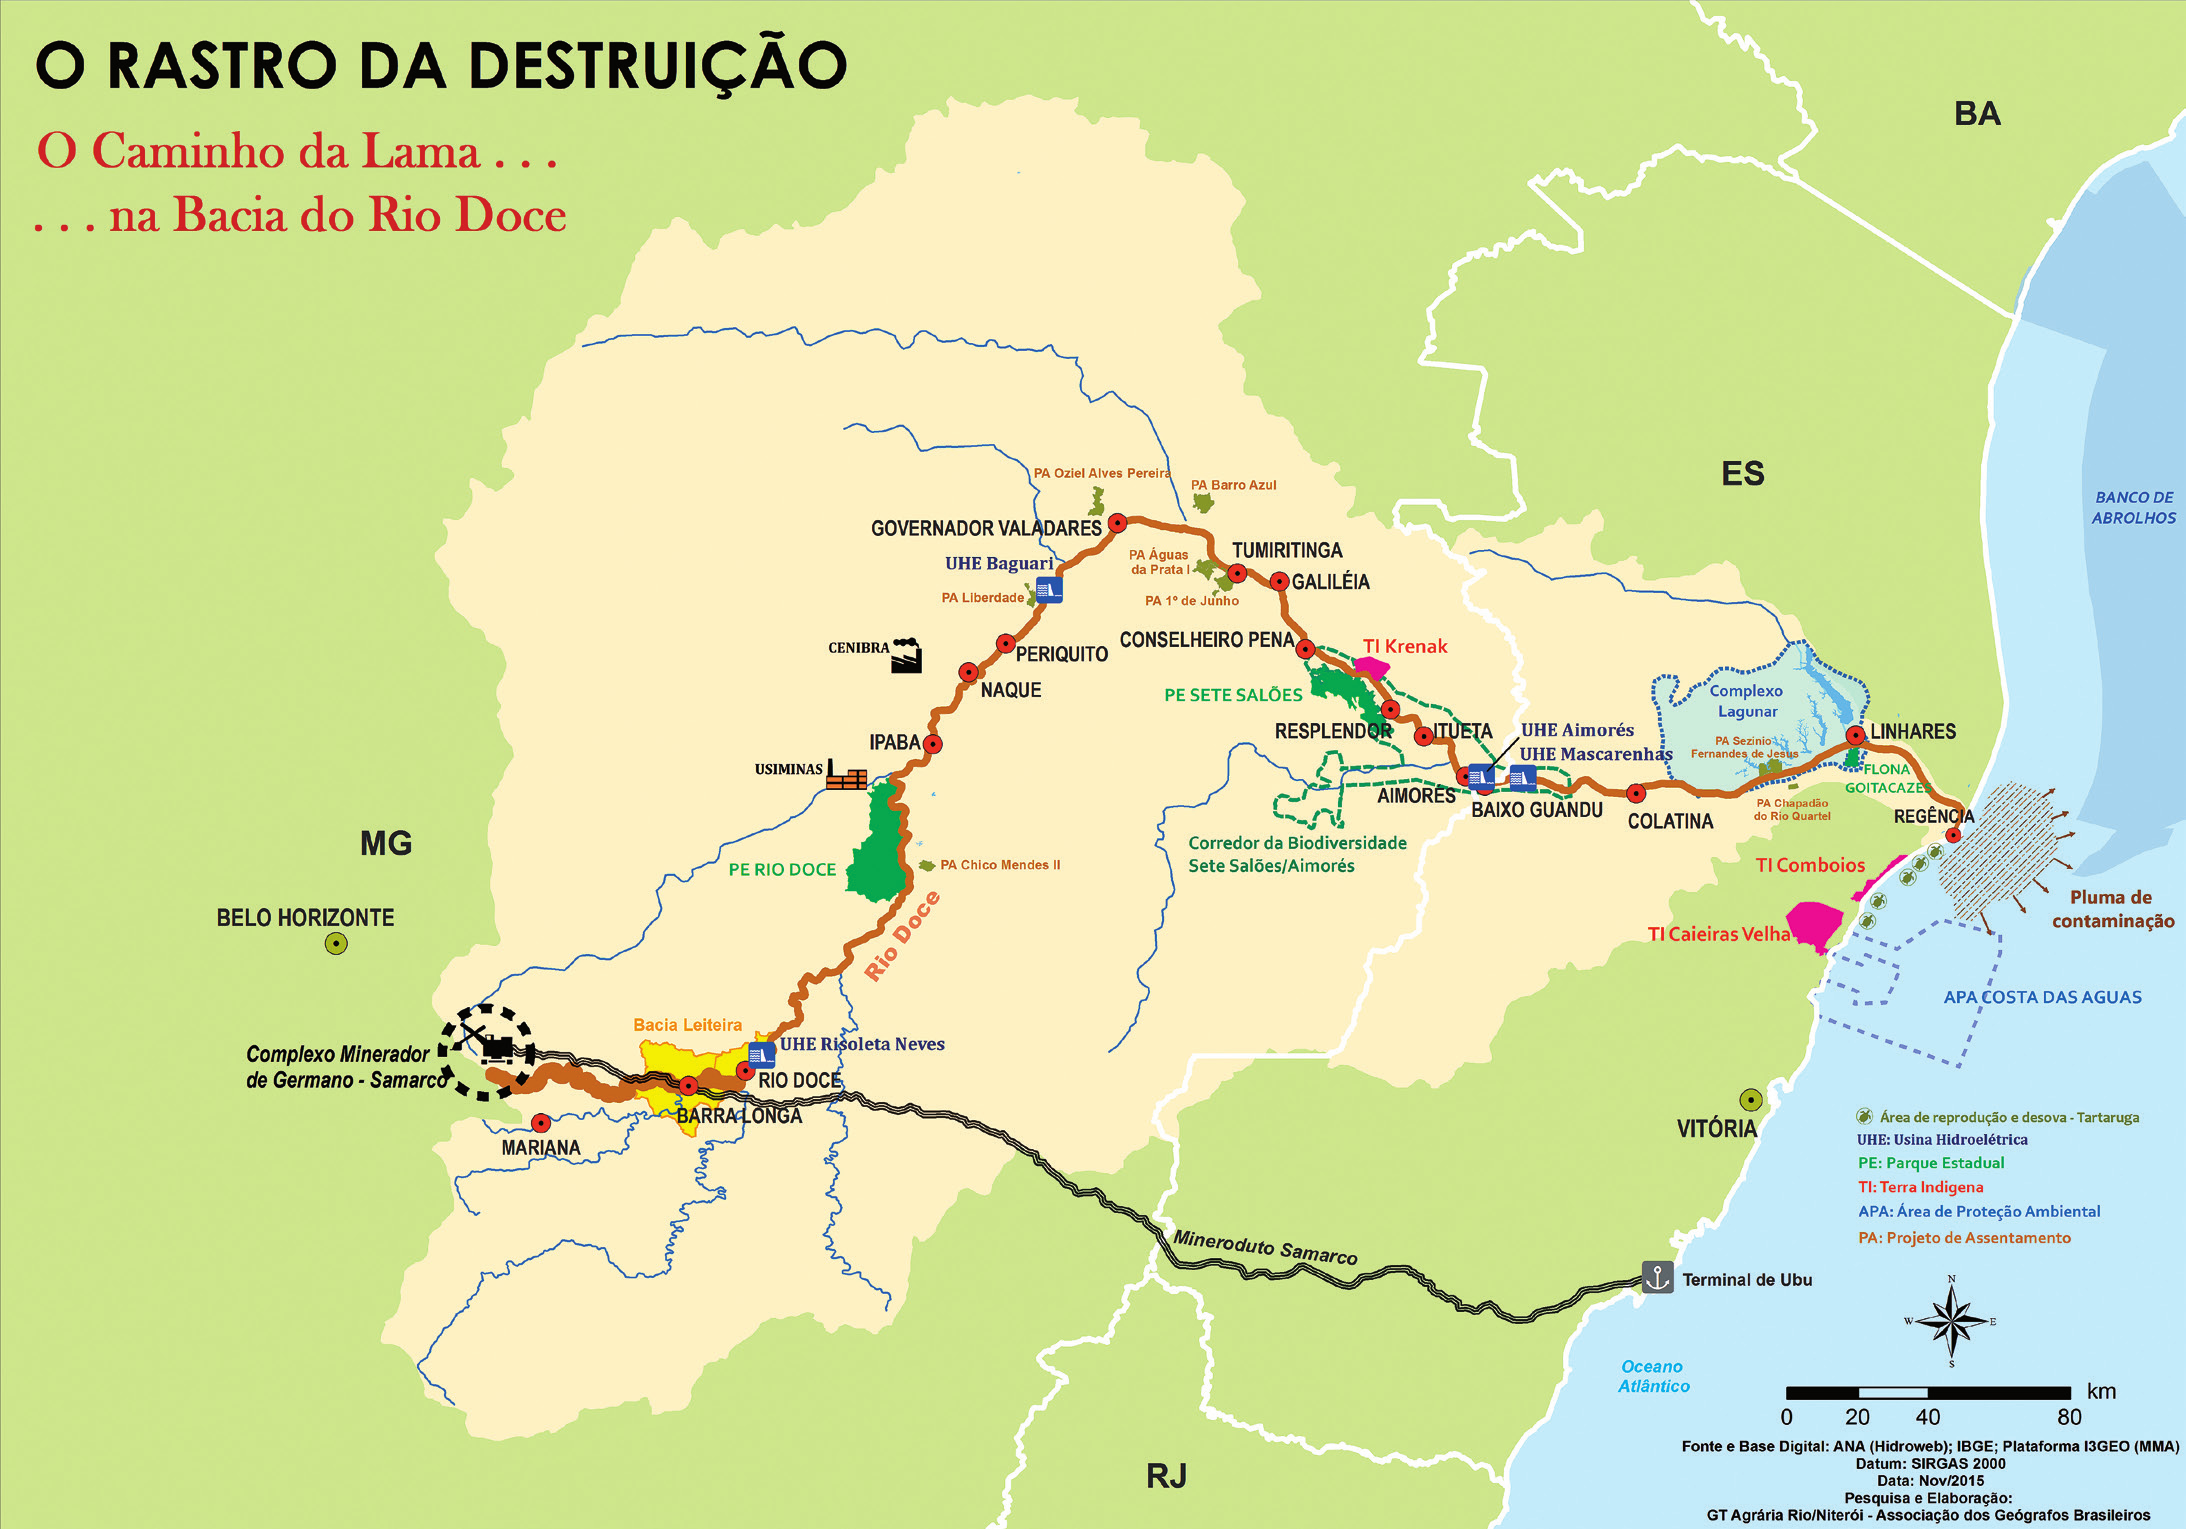
\includegraphics[width=1.0\linewidth]{img/pinto_005_01.png}
		\legend{Reproduzido de \citeonline[p.34]{wanderley2016a}}
		\label{fig:mapalama}
	\end{figure}
	 
	Em seu caminho (vide \autoref{fig:mapalama}), a lama arrastou a vegetação, animais e entulho por uma área de extensão de 663 km até o mar, embora o maior impacto tenha se concentrado entre os municípios de Mariana e Rio Doce, no qual a Usina Hidrelétrica Risoleta Neves reteve uma parte dos detritos. A lama atingiu o Rio Gualaxo do Norte e o Rio do Carmo até chegar no Rio Doce, alterando o PH do solo e das águas com aminas tóxicas utilizadas no processo de flotação catiônica. Dezenove pessoas perderam a vida como resultado do rompimento das barragens, e no mês seguinte, onze toneladas de peixes mortos foram retiradas dos rios atingidos \cite{lopes2016a}.
	 
	Quase quatro anos depois, a perda de biodiversidade parece incalculável, o Rio Doce foi declarado morto e a população ribeirinha ainda sofre consequências ambientais e socioeconômicas. Enquanto isso, a Vale S.A., responsável pelo controle da mineradora Samarco em uma \textit{joint-venture} com a australiana BHP Billiton Brasil Ltda., obteve lucro líquido de R\$ 25 bilhões no ano de 2018 \cite{glauce2019a} \cite{sudre2019a}, período no qual atingiu o valor de mercado de aproximadamente R\$ 300 bilhões \cite{sudre2019a}.
	 
	As multas ambientais aplicadas pelo \gls{ibama} são contestadas pela mineradora, que pagou apenas aproximadamente um terço  do exigido pela \glsdesc{semad}. A ação civil pública proposta pelo Ministério Público Federal e ação promovida pela União e pelos estados atingidos foram suspensas pela Justiça Federal mediante acordo feito com a Samarco em agosto de 2018 \cite{rodrigues2019a}. Em Janeiro de 2019, rompeu-se  a barragem de rejeitos de outro empreendimento de mineração da Vale S.A., desta vez no município de Brumadinho (MG), na região do Córrego do Feijão, com consequências catastróficas, mais perda de biodiversidade e mortes, desta vez mais de 200 pessoas perderam a vida.
	 
	Em ambos os empreendimentos, as barragens de rejeitos continham restos de elementos minerais além de aminas utilizadas no processo de flotação de rejeitos, necessário para a separação do minério de ferro impuro. Após longo período de extração intensa, os minerais com maior nível de pureza foram se esgotando, a flotação catiônica é a solução utilizada há décadas pela Vale, a adição de amidos age precipitando o minério de ferro, enquanto as aminas causam a flotação da ganga. Somemos esta prática potencialmente poluidora utilizada em empreendimentos inseguros e que têm sua capacidade excedida, a um investimento relativamente baixo em manutenção da infraestrutura, resultante de uma busca frenética por lucros cada vez mais vultosos, e teremos a receita pronta para o desastre.    
	 
	Desde a solicitação para a construção da barragem pela mineradora em 2007, o processo de licenciamento foi permeado de omissões por parte do poder público e da própria empresa, que conseguiu autorização para iniciar as obras em um curto período  de três meses, em contraste com processos de licenciamento ambiental que costumam ser demorados. Ao menos desde 2014 a empresa estava ciente dos riscos de rompimento e decidiu manter a operação do empreendimento sem tomar as medidas necessárias, segundo autoridades \cite{santos2018a}.

	\section{De que modo os ciclos biogeoquímicos foram afetados?}
	% Responsável: Anselmo
	
	A Constituição Federal Brasileira, em seu Artigo 225 estabelece que todos têm direito ao meio ambiente ecologicamente equilibrado \cite{brasil1988a}, contudo é recorrente a violação de direitos humanos e constitucionais pelas ações negligentes de corporações de empreendimentos que apresentam risco ambiental incomensurável como ficou constatado pelos eventos trágicos, mas infelizmente não surpreendentes ocorridos na tarde de 05 de novembro de 2015, o equilíbrio ambiental foi desnorteado com o rompimento da Barragem de rejeitos de mineração de Fundão, em Mariana (MG), mas não se restringindo a ela, impactando 39 municípios localizados à jusante do Rio Doce.
	
	O crime ambiental descrito no presente artigo afetou diretamente a interação entre os seres vivos e o ambiente; certamente são diversas as espécies locais de microrganismos, peixes, insetos e outros animais que foram extintas\footnote{Vide \autoref{ss:dinamica} e \autoref{s:comportamento}}, ademais, poderíamos mencionar a forte possibilidade de que tenha ocorrido uma redução ou até extermínio de espécies que nem chegaram a ser cientificamente catalogadas.
	
	Mas como uma alteração nas interações das espécies poderia afetar uma mudança no fluxo de energia e de matéria do ambiente de estudo?
	
	Primeiramente, a vegetação coberta pela lama não é capaz de realizar fotossíntese, isto é, usar luz do sol, água e gás carbônico atmosférico, a base da cadeia alimentar e consequentemente da cascata trófica foi comprometida, pois a maioria dos seres vivos não é capaz de sintetizar o próprio alimento como fazem as espécies fotossintetizantes. 
	
	É possível deduzir como funcionava naturalmente a entrada de energia no sistema, ou melhor,  como funcionava o ciclo de energia no ambiente impactado: os grandes produtores são as espécies vegetais às margens dos rios e nas florestas, além do fitoplâncton na água. Esses produtores são predados por diversos consumidores primários, passando a energia presente na glicose, sintetizada pela energia solar, água e matéria inorgânica, impulsionando o fluxo de energia de um organismo para a espécie consumidora. Essa teia alimentar também inclui consumidores secundários, tais como peixes, répteis e outros, consumidores terciários (p. ex., cobras e mamíferos maiores) e decompositores, entre os quais as bactérias, fungos e outros microrganismos.
	
	Com o rompimento da barragem, a lama levou para a jusante do rio não apenas carros, casas e vidas humanas, mas também uma gama de seres vivos foram arrastados juntamente com o material orgânico presente na serapilheira das florestas impactadas, bem como o banco de sementes ali presente, comprometendo assim a possibilidade de regeneração natural das espécies vegetais presentes no local e com ela, o fluxo de matéria no ambiente. 
	
	O fluxo de matéria ficou comprometido pois com a eliminação de espécies vegetais as folhas e sementes deixam de ser depositadas no solo, com isso, não há material orgânico para se decompor e devolver ao solo os nutrientes repostos naturalmente quando o ambiente estava dentro da zona de equilíbrio. Após a lama arrastar vegetais, poluir as águas e cobrir toda a superfície do solo com minerais tóxicos ou exóticos ao local, não há possibilidade dos ciclos biogeoquímicos principais serem realizados, todo o ambiente foi colapsado: nitrogênio, carbono, enxofre, oxigênio e até mesmo água tiveram suas dinâmicas impactadas.
	
	O comprometimento dos ciclos biogeoquímicos pode parecer algo simples e até mesmo não importante, no entanto, é preciso lembrar que os elementos químicos não estão isolados na natureza, o carbono, oxigênio, hidrogênio, nitrogênio e fósforo podem até mesmo ser tratado como passivos ambientais causadores de poluição, efeito estufa e eutrofização de ambientes aquáticos, mas é necessário lembrar que graças a eles, moléculas simples ou complexas, essenciais para a manutenção da vida na Terra são formadas: água, carboidratos, proteínas e \gls{dna} \cite{ricklefs2016a}.
	
	\section{Como as comunidades ecológicas da bacia do Rio Doce foram afetadas?}
	
	Os danos causados na Bacia do Rio Doce após o rompimento da barragem de rejeitos da operação mineradora da Samarco foram vastos e visíveis, contudo ainda é cedo para determinar os impactos causados, inicialmente abordar-se-á como as comunidades locais foram impactadas.
	
	O efeito destrutivo do escorrimento da lama foi um assolamento das comunidades terrestres do entorno, como a lama extrapolou a calha dos rios Gualaxo do Norte, Carmo e Doce. Depois de encaminhar-se no Rio Doce, os rejeitos que incluíam lama e detritos orgânicos foram parcialmente detidos pela barragem da \gls{uhe} de Candonga, depois disso a lama ainda seguiu o curso do Rio Doce, mas dentro de sua calha principal.
	
	A lama não destruiu e arrancou apenas árvores e vegetação herbácea, na realidade carregou e soterrou a serapilheira, que é a camada formada pela deposição dos restos de plantas e acúmulo de material orgânico vivo em diferentes estágios de decomposição que reveste superficialmente o solo ou o sedimento aquático, e seus bancos de sementes, então houve um enorme prejuízo e comprometimento de resiliência e dos processos de sucessão ecológica. Essas comunidades que inicialmente colonizaram a região sofrem por processos de alteração, adaptação e sucessão ecológicas que são esperados e naturais, mas o desastre ambiental causado pelo rompimento da barragem afetou as comunidades ecológicas de modo que extrapolou os limites de resiliência ecossistêmica do local e em um efeito cascata desconfigurou a dinâmica inter-comunidades da área e das que estão conectadas à ela.
	
	Um dos fatores que ainda precisam ser avaliados e estudados é a contaminação dos alimentos, por metais pesados, por exemplo. \citeonline[p.141]{scotti2015a} sumariza o tipo de processo adotado pela Samarco:
	
	\begin{citacao}
		``A flotação catiônica reversa tem sido utilizada pela Samarco desde o final da década de 1970. Este sistema ocorre em meio aquoso, consistindo na precipitação do minério de ferro e flotação do material restante na ganga (rejeito) [\dots] Para que tal separação ocorra, alguns reagentes devem ser adicionados ao sistema. Os principais deles são o amido, utilizado como depressor dos minerais de ferro, e as aminas (éter mono-amina e éter di-aminaque) que são os únicos coletores catiônicos usados industrialmente.
		
		[\dots]

		A reação de flotação reversa ocorre em pH alcalino, geralmente entre 10 e 10,5. Sob essas condições, a sílica apresenta carga negativa e a amina é absorvida na superfície do quartzo, formando uma espuma, a qual é removida na parte superior das máquinas de flotação e constitui o rejeito de mineração.''
	\end{citacao}
	
	Segundo \citeonline[p.146]{scotti2015a}, uma série de visitas e análises técnicas a partir de diferentes relatórios produzidos por órgãos do poder público, entre eles \gls{ibama} e \gls{semad}, viabilizou a compilação de uma lista de impactos ambientais, dos quais destacamos:
	
	\begin{itemize}
		\item Acúmulo de sedimentos instáveis nas margens, com potencial erosivo;
		\item Contaminação química por éter-aminas com toxicidade potencial;
		\item Contaminação por arsênio, ferro, manganês, cobre, chumbo, magnésio e alumínio, metais estes em valores superiores aos estabelecidos na legislação \apud[p.146]{brasil2005a}{scotti2015a};
		\item Perda drástica de biodiversidade da fauna e flora (não quantificada quando da publicação do artigo).
	\end{itemize}
	
	% TODO a fonte não foi citada no final
	O possível surgimento de zoonoses com o aumento de contato entre pessoas, animais domésticos e silvestres que vão sobrepor as áreas de uso na busca de alimento, abrigo e água nos habitats restritos que se mantiveram de alguma forma a salvo. É importante observar o tempo e a capacidade de depuração dos elementos que foram despejados no solo e nas águas, o surgimento dos novos compostos químicos na dinâmica ecossistêmica e a composição de sucessão ecológica na área atingida, possivelmente com uma invasão de espécies, inclusive exóticas. Segundo \citeonline[p.123]{delpupo2015a}, ``o soterramento concomitante do solo, banco de semente e plantas mais jovens ou de menor porte, comprometeu severamente a sucessão vegetal''. 
	
	\begin{citacao}
		``Segundo um levantamento feito pela EMBRAPA, a lama depositada
		ao longo das margens dos rios dificilmente poderá transformar-se
		em um solo estruturado que permita uma sucessão ecológica
		natural que restabeleça as comunidades vegetais, originalmente
		presentes nessas regiões (INSTITUTO BRASILEIRO DO MEIO
		AMBIENTE E RECURSOS NATURAIS RENOVÁVEIS, 2015).'' \cite{pinto2015a}
	\end{citacao}
	
	Supondo que ocorra um processo de seleção dos indivíduos sobreviventes do desastre, supomos que alguns peixes têm um gene que os permite resistir ao envenenamento por metais pesados e rapidamente essa comunidade de peixes consegue se adaptar às novas características da bacia, logo animais que predam essas espécies aquáticas começariam a passar por um processo semelhante, então quanto tempo levaria para essa cascata ecológica chegar no impacto da população humana que depende da pesca, da agricultura e da pecuária da região?
	
	Pode-se ainda dizer que o impacto que está sendo causado, muito dele ainda não identificado, à espécie humana, indo desde a contaminação de alimentos à proliferação de vetores de doenças como muito mais do que uma catástrofe ambiental, é um crime não somente contra o meio-ambiente, mas também à vida humana. Suponhamos, por exemplo, que aconteça um assentamento dos rejeitos às margens de uma região do rio principal ou de seus afluentes de modo que dificulte a reprodução dos anfíbios e aracnídeos que predam mosquitos, incluindo o \textit{aedes aegypti}, devido a redução drástica de predadores, a população de mosquitos sofra um aumento substancial e consequentemente seja registrada uma epidemia de dengue ou malária na região, neste cenário drástico, quem é responsável pelo impacto e pelas possíveis mortes? Não se pode ignorar a participação das ações da Samarco e de suas subsidiárias no impacto que a vida na região vai sofrer pelos próximos meses e anos, que incluem perdas incalculáveis para a biodiversidade e para as comunidades ecológicas e humanas do local.
	
	\section{Qual foi o impacto real sofrido pelas populações ecológicas da bacia do Rio Doce?}
	
	Segundo \citeonline{ricklefs2003a} populações podem ser compreendidas como a consistência de muitos organismos de uma mesma espécie vivendo em um mesmo local.
	
	Um certo nível de seleção e adaptações são intrínsecas à evolução da vida em um habitat, contudo o crime ambiental cometido pela Samarco em Mariana extrapolou em muito o processo evolutivo, não se restringindo à espécies isoladas, mas impactaram a sociedade e o ecossistema agressivamente.
	
	Para compreendermos a extensão dos danos, que vão desde o rompimento da dinâmica populacional até a extinção de populações ecológicas inteiras, é oportuno agrupar a lista de espécies conforme reportagem de \citeonline{calixto2016a}, que sustenta que, de acordo com Ibama (2015), após um mês do rompimento das barragens, a análise da área afetada pelos rejeitos de minério da barragem, pode chegar a 400 o número de espécies impactadas, sendo 3 espécies de plantas ameaçadas, 4 espécies de répteis, 28 espécies de anfíbios, 35 espécies de mamíferos,  64 a 80 espécies de peixes e 112 a 248 espécies de aves, totalizando entre 246 e 398 espécies. A reportagem ainda considera que a situação mais crítica é a dos peixes:
	
	\begin{citacao}
		``A situação mais extrema é a das espécies de peixes. Segundo o laudo, o Rio Doce tinha onze espécies ameaçadas de extinção, incluindo quatro definidas como 'Criticamente em Perigo'. Dessas, duas são endêmicas, só existem no Rio Doce, e portanto podem desaparecer. Ao todo, havia 12 espécies endêmicas na área afetada. Esses peixes são os que mais estão em perigo.'' \cite{calixto2016a}
	\end{citacao}
	
	O referido laudo chama a atenção para três espécies de plantas ameaçadas da região que foram soterradas pela lama: \textit{Dalbergia nigra} (jacarandá-cabiúna), \textit{Melanoxylon brauna} (braúna) e \textit{Euterpe edulis} (palmito). A lama destruiu de 1.469 hectares de mata nativa, incluindo áreas de preservação permanente. As populações animais têm menores chances de se extinguir devido à mobilidade, mas plantas e fungos sofreram consequências mais severas.
	
	Ainda que muitas áreas apresentassem as mesmas espécies, é importante destacar que há variação genética entre populações devido ao isolamento de espaço geográfico. Imaginemos que uma população de Dalbergia nigra, o jacarandá-cabiúna de um lado da margem de um rio vai sofrer alterações e ser naturalmente selecionado para apresentar resistência à uma praga, mas a população na outra margem do rio não apresentava a característica, ainda que sejam a mesma espécie, a variabilidade genética permite que uma determinada sub-população apresente vantagens evolutivas consequentes das contínuas adaptações e seleção.
	
	\subsection{Como funcionava a dinâmica e as estruturas populacionais na bacia antes da tragédia de Mariana e o que mudou?} \label{ss:dinamica}
	
	A estrutura populacional contempla a organização das características genéticas e demográficas de uma espécie e as mudanças e sucessivas adaptações pelas quais os organismos passarão.
	
	O que determina o aumento ou diminuição de análise populacional são os parâmetros populacionais, portanto o tamanho populacional sofre influência do número de indivíduos da população através dos parâmetros que caracterizam aumento populacional quando relevante imigração somado a taxa de nascimento quando concatenados; já a diminuição populacional é caracterizada diante da emigração agregada a taxa de mortalidade populacional.
	
	O crescimento populacional se caracterizará por ser exponencial e logístico, podendo ser o exponencial contínuo ou discreto.
	
	Conforme dados abordados, a destruição da população e da vegetação nativa de mata atlântica caracteriza a mortandade de biodiversidade aquática e terrestre com extermínio inclusive de populações planctônicas, invertebrados aquáticos, além de peixes, anfíbios, répteis e mamíferos que se beneficiaram dos recursos do Rio Doce.
	
	A lama se depositou nos interstícios dos grãos de areia e isto consequentemente prejudicou a vegetação que ocupava a região, extrapolando os limites de resiliência. Vale destacar que a alteração do solo é praticamente irreversível.
	
	A população às margens do Rio Doce sofreram além do desmatamento, causado pelas alterações físico-químicas do solo, impactos na flora que por sua vez afetarão a fauna e prejudicando drasticamente a cadeia trófica.
	
	A bacia hidrográfica do Rio Doce foi forçadamente reestruturada, até então permissiva em biodiversidade, rica em espécies, composta por 98\% do bioma Mata Atlântica, insetos polinizadores, bichos dispersores e predadores potenciais, muda não somente em mortandade da ictiofauna, mas também desestrutura a Zona Estuarina do litoral do ES, local importante de desova de tartarugas marinhas.
	
	Entre as mortes daquelas 11 toneladas de peixes da Bacia do Rio Doce, das mais diversas espécies deste habitat, é preciso dar um destaque especial para carás, lambaris, bagres, traíras, que são espécies mais resistentes, e começaram a retornar para o leito do rio.
	
	A migração esperada que ocorreria no período de desova dos peixes da bacia, que costumava iniciar-se em Piracema, mesmo não afetando diretamente o número de peixes mortos, afetará o recrutamento, a lama atingiu os peixes em momento importante e comprometeu a reprodução.
	
	Entre os peixes migratórios nativos do Rio Doce estão o piau-vermelho, piau-branco e as ameaçadas de extinção piabanha e curimatã. Também o dourado, o curimba-do-são francisco e surubim, que são exóticos, e foram introduzidos na bacia para que subam para desova.
	
	Oito espécies sofrem risco de extinção: andirá, surubim-do-doce, curimatã, timboré, piabanha, pirapitinga, lambari bocarra, e o cascudinho. A situação destes peixes se agrava, uma vez que boa parte deles é natural do alto do Rio Doce, próximo ao Rio Piranga, uma das áreas mais afetadas pelo lamaçal. Especialmente surubim-do-doce, curimatã e piabanha, sendo as duas últimas migratórias. 
	
	Há conjectura amoral do comportamento do homem, comportamento que vem provocando a destruição de biomas naturais ou no mínimo os marcando de modo irreversível, que é o caso de crimes como o que foi cometido no vale do Rio Doce, ecossistema que assiste o descaso e desapego da não evolução e desrespeito social e crueldade em seu meio ambiente.
	
	Imaginar a quantidade populacional de espécies não descobertas neste ambiente  remete a uma estagnação de avanços medicinais e científicos  por parte deste ecossistema, que recebe ajuda de organizações filantrópicas de todo Brasil, além de professores e profissionais das diversas áreas biológicas que gritam por medidas resilientes por parte da Mineradora Vale do Rio Doce juntamente com o Estado Brasileiro.
	
	\section{Qual é o comportamento social dos organismos?} \label{s:comportamento}
	% Responsável: Caio César
	
	Conforme \citeonline[p.401]{odum1990a}, a conduta social pode ser observada quando há ``uma rede de comunicações, alguma forma de hierarquia de domínio, aprendizagem e um equilíbrio entre condutas contraditórias'', sendo que as condutas contraditórias podem ser competição versus cooperação ou agregação versus isolamento, por exemplo e, sendo que a organização pode ser monoespecífica (quando envolve indivíduos da mesma espécie) ou poli-específica (quando envolve várias espécies).
	
	Num contexto de desastre, como elucida \apudonline[p.6]{kreps2001a}{carmen2012a}, são afetados os sistemas sociais, envolvendo múltiplas escalas e dimensões (da menor até níveis mais abrangentes), não deixando de estar ``interligados à incerteza e a uma inevitável dinâmica  de  mudança;  correspondem  a  eventos  não rotineiros nas sociedades que envolvem disrupção social e  danos  humanos''. Ainda e, mais alarmante ainda é a consideração de \apudonline[p.6]{perry2001a}{carmen2012a}, que considera que os desastres catalisam fisicamente e socialmente a ação coletiva, antes, durante e depois.
	
	Quando \citeonline[p.160]{ricklefs2003a} introduz a temática envolvendo o comportamento social das espécies, fica subentendido que se trata de um intrincado processo, que inclusive envolve a alternância entre variedades de uma mesma população, resultando no que o autor resume como uma ``ciclagem nas frequências dos três morfos''. Trata-se de um conceito que permite que suscitemos reflexões sobre o impacto dos recentes crimes ambientais ocorridos no estado de Minas Gerais. Como \citeonline[p.161]{ricklefs2003a} salienta, ``durante o curso de sua vida, cada indivíduo interage com muitos outros da mesma espécie: parceiros, filhotes, outros parentes e membros não aparentados de seu grupo social''. Por exemplo, sabe-se que as bacias hidrográficas foram duramente atingidas, com grandes cursos hídricos, como o Rio Doce, tendo a composição das águas e o ecossistema consideravelmente alterados, neste sentido, fatores como a territorialidade podem ter se tornado impraticáveis, devido à ``efemeridade de recursos críticos'' \cite[p.162]{ricklefs2003a}. A \autoref{fig:grupos} exemplifica casos de comportamentos sociais para vida em grupo, com suas vantagens e desvantagens.
	
	\begin{figure}
		\centering
		\caption{Vantages e desvantagens da vida em grupo em bandos do pintassilgo-comum}
		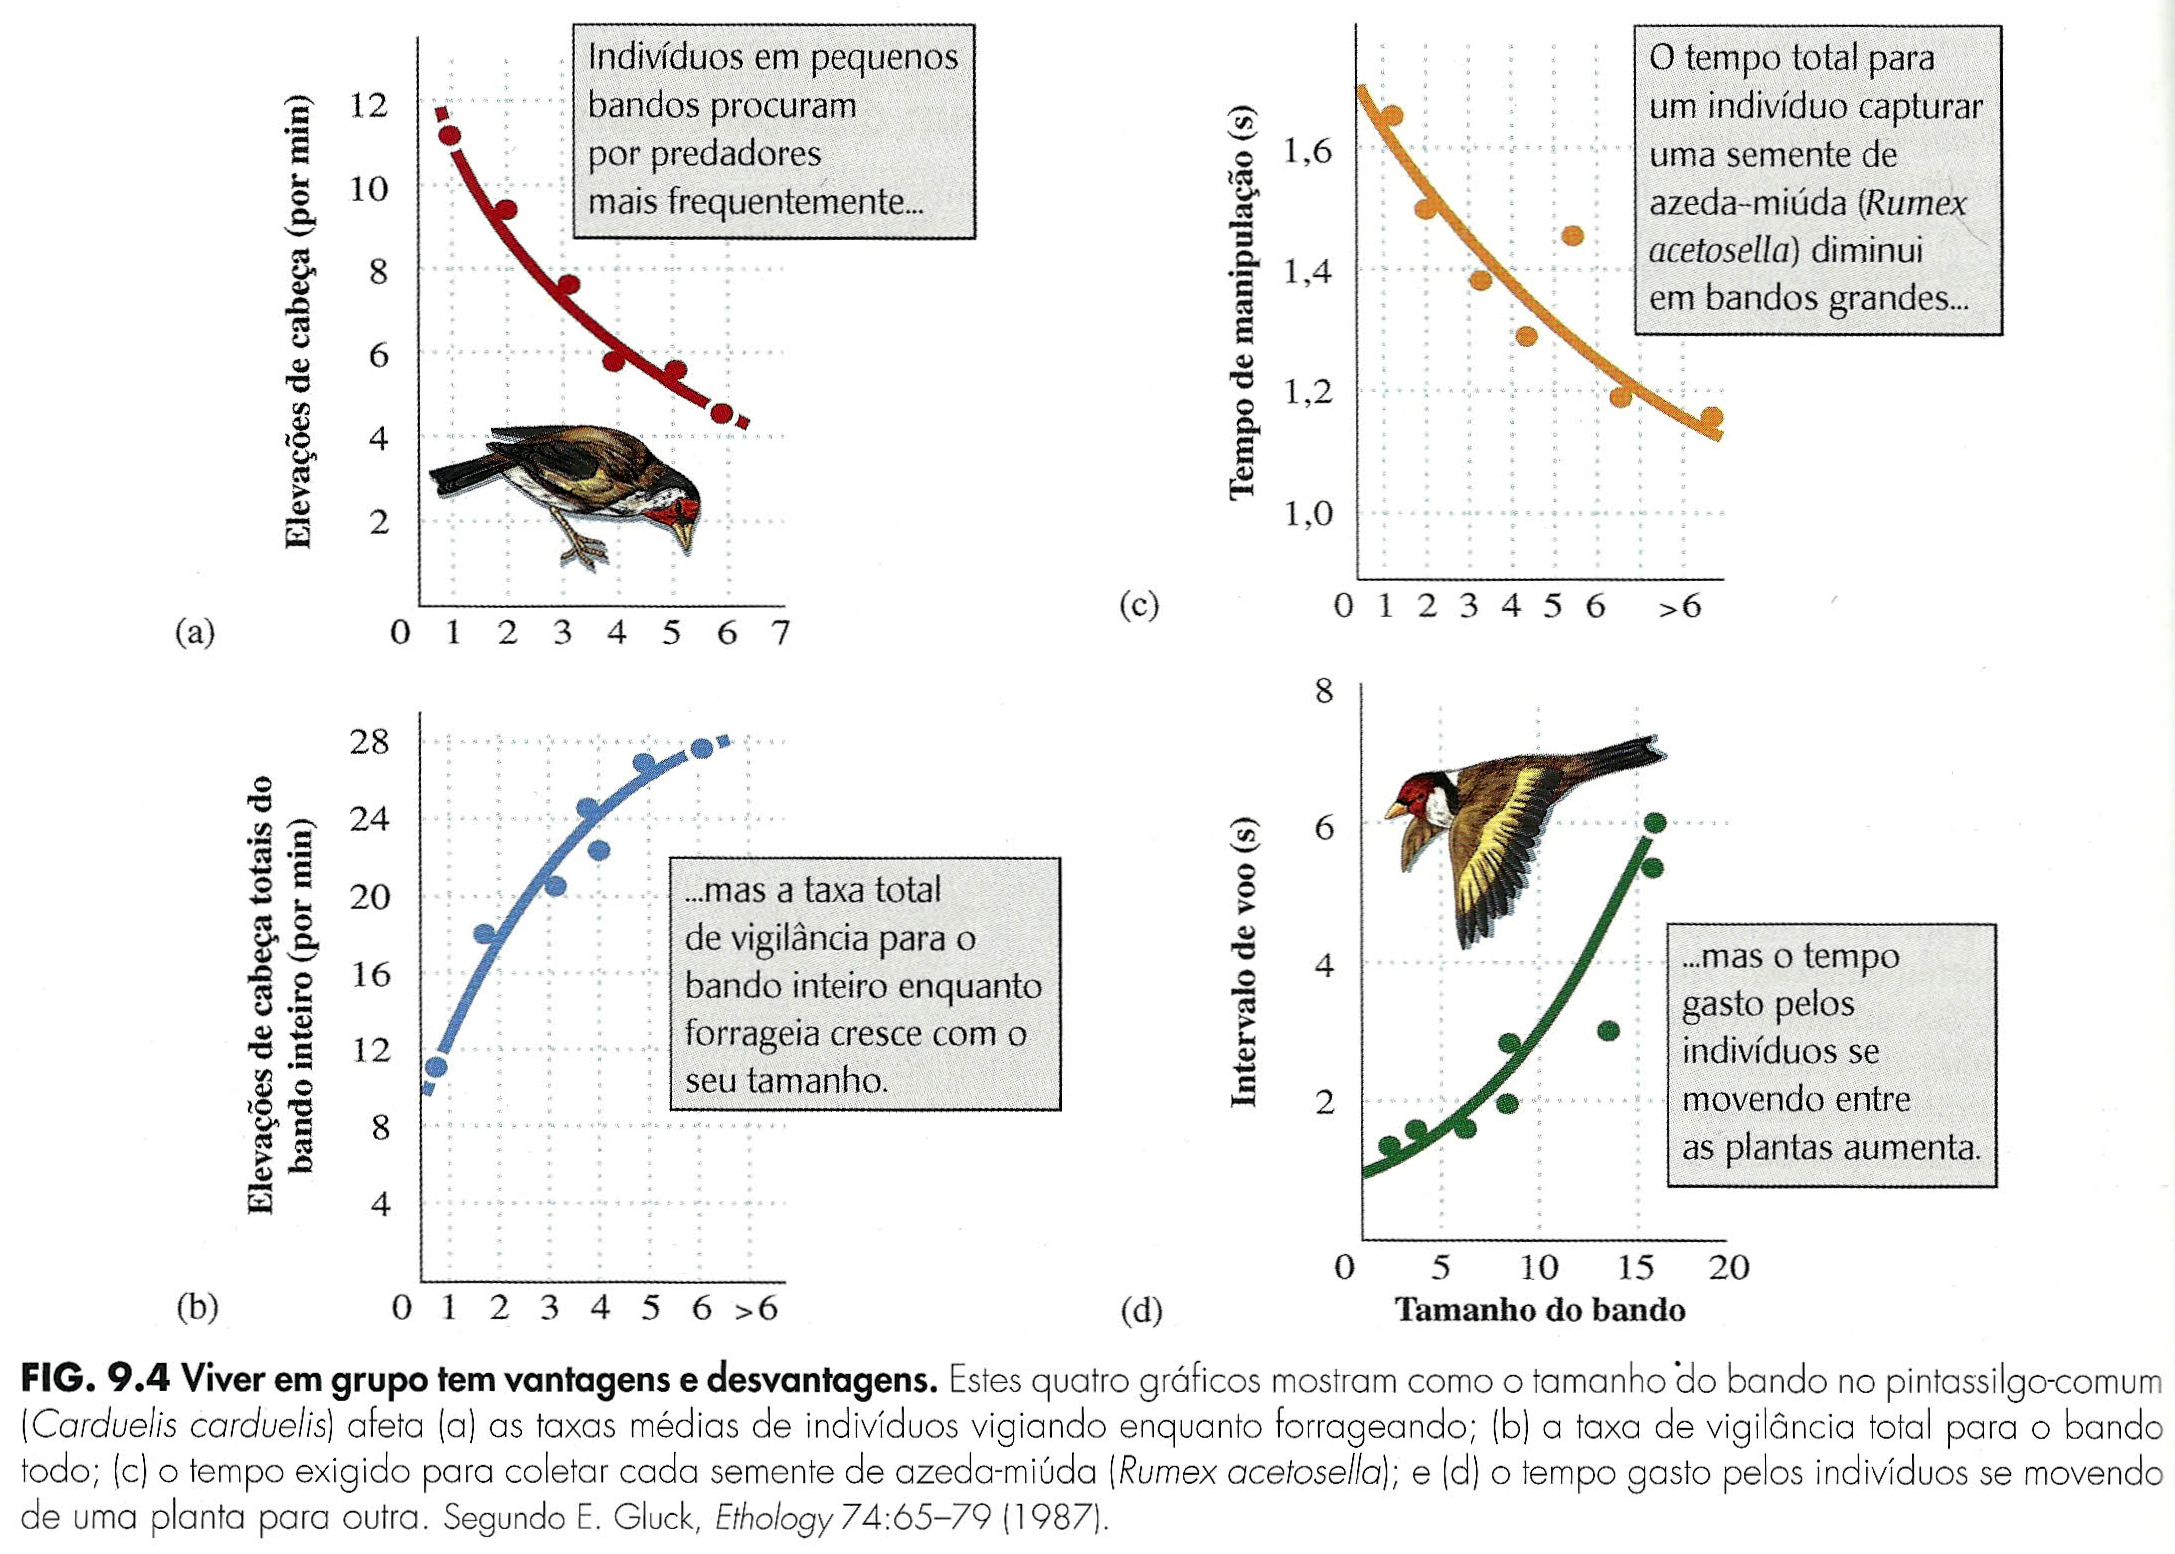
\includegraphics[width=1.0\linewidth]{img/rick_180_01.png}
		\legend{Reproduzido de \citeonline[p.164]{ricklefs2003a}}
		\label{fig:grupos}
		
		\caption{Abrangência demográfica de uma população e sua relação com a ocupação de habitats adequados}
		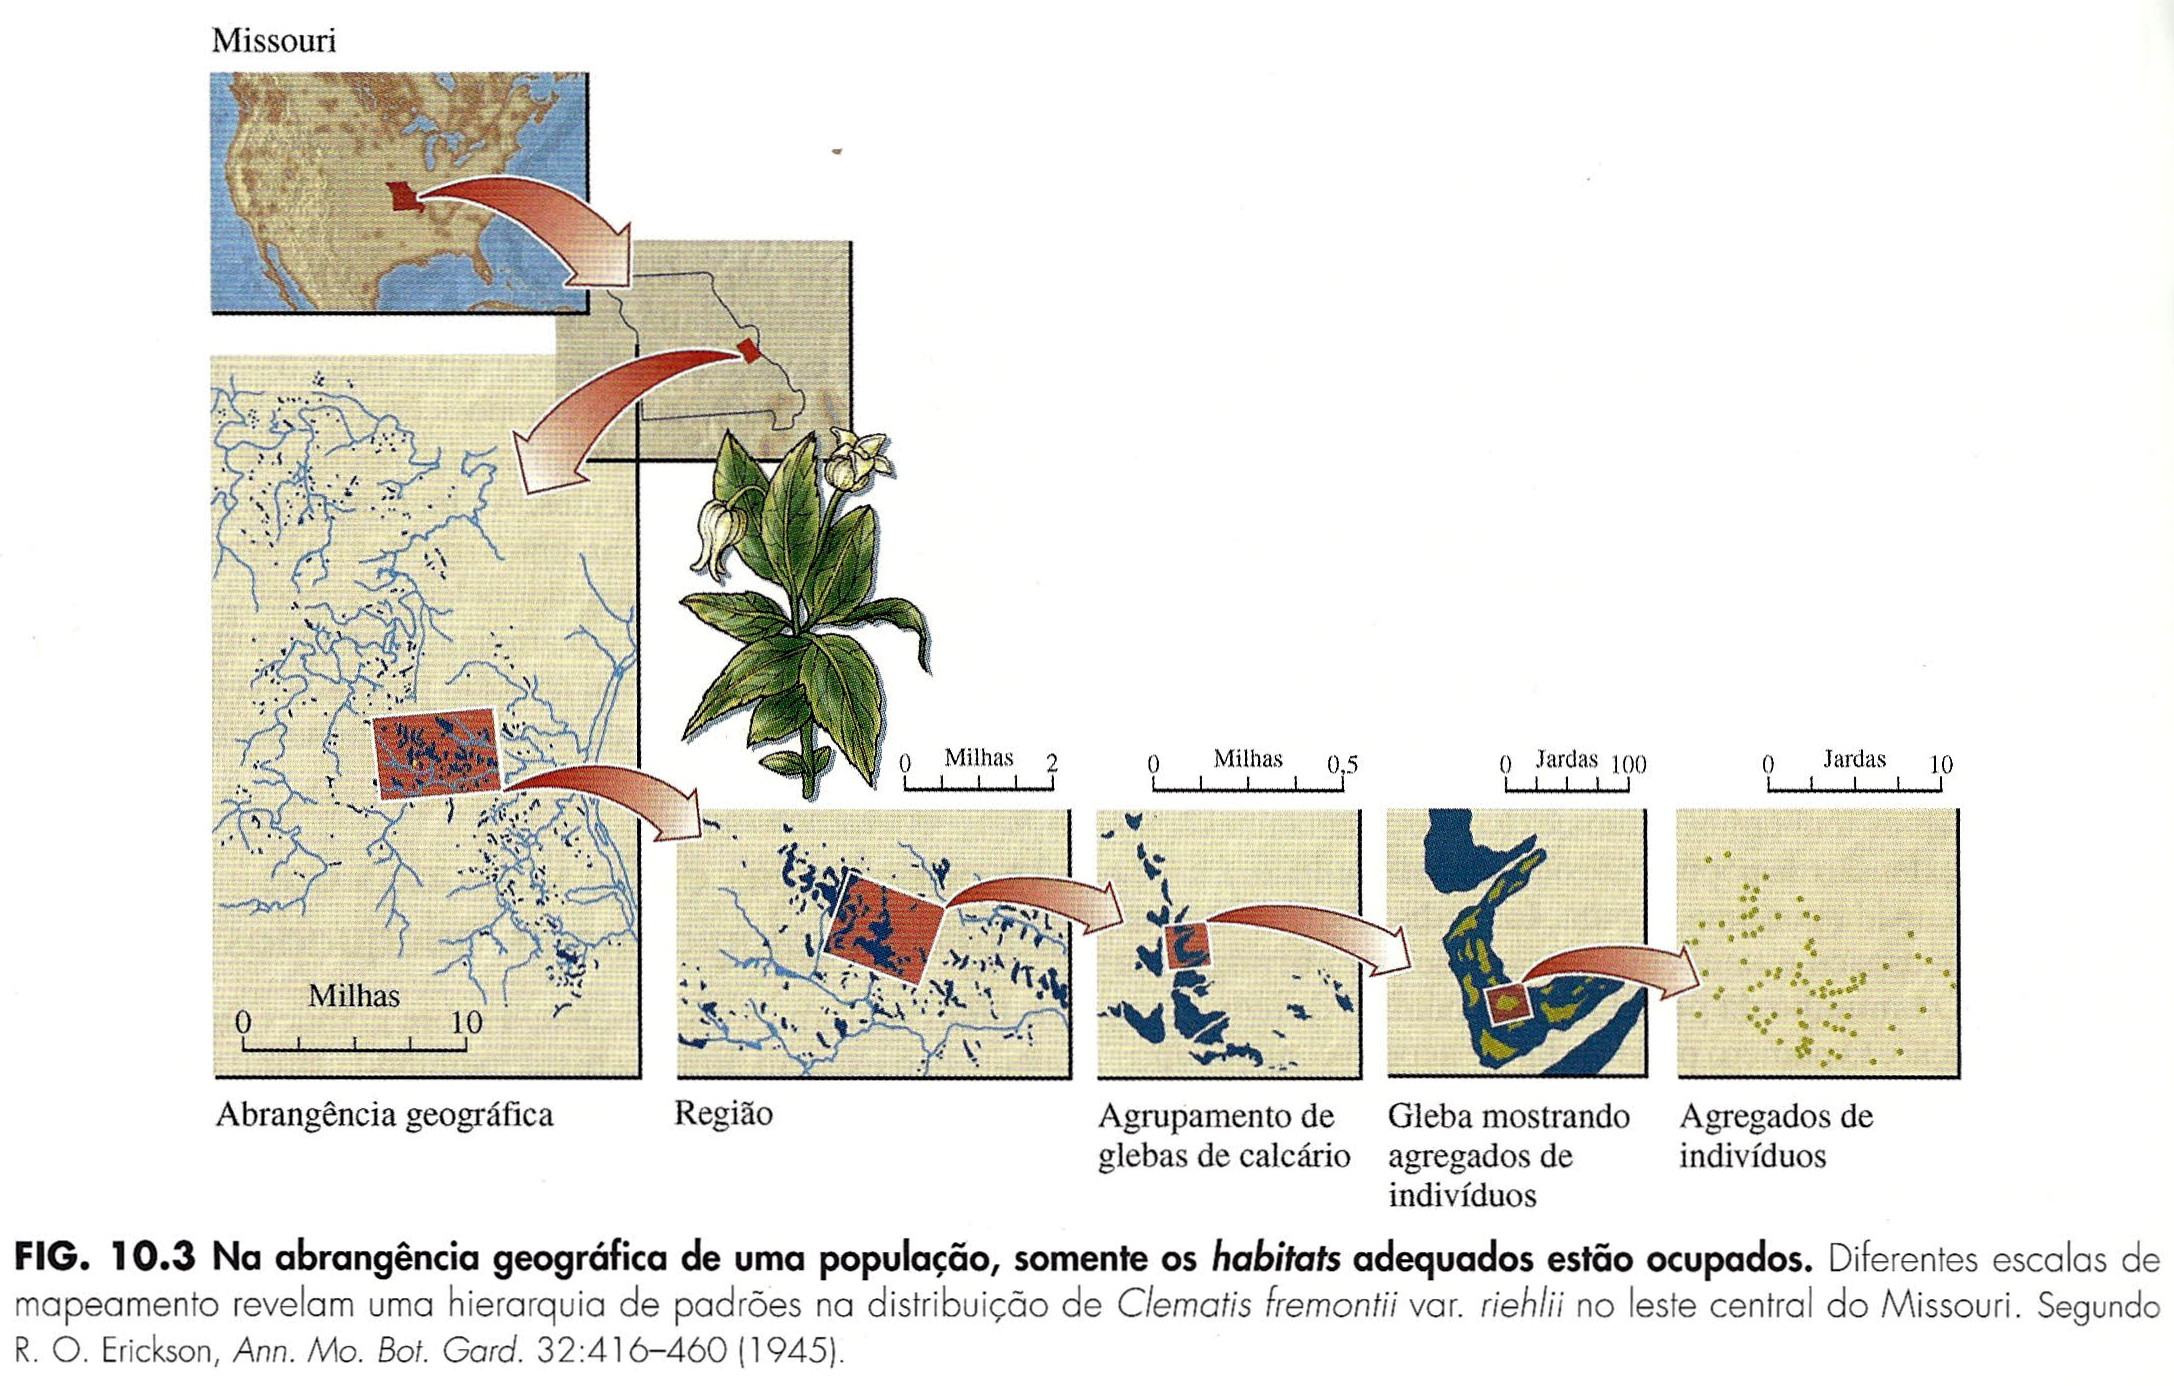
\includegraphics[width=1.0\linewidth]{img/rick_194_01.png}
		\legend{Reproduzido de \citeonline[p.178]{ricklefs2003a}}
		\label{fig:habitats}
	\end{figure}
	
	Ainda sobre a bacia hidrográfica, para \citeonline[p.7]{lopes2016a}, ``os efeitos dramáticos e perversos do `desastre de Mariana' serão sentidos por décadas e gerações, principalmente aquelas formadas por comunidades que estão localizadas dentro da bacia hidrográfica do Rio Doce'', além disso, \citeonline[p.12]{lopes2016a} também salienta que a mesma bacia ``agoniza a espera de ações que minimizem os danos causados ao seu ecossistema''.
	
	\subsection{Qual a dinâmica por trás da disputa territorial dos organismos?}
	
	Primeiramente, faz-se necessário conceituar a existência de dois tipos de intervalos de condições para existência de populações: \textbf{nicho fundamental} e \textbf{nicho percebido}. O primeiro diz respeito ao ``intervalo de condições físicas dentro do qual as espécies podem persistir'' \cite[p.177]{ricklefs2003a}, enquanto o segundo diz respeito a um intervalo menor, limitado por ``predadores, patógenos e competidores'' \cite[p.177]{ricklefs2003a}. Outro aspecto nevrálgico é manter em perspectiva que ``\textit{habitats} uniformes se estendendo por grandes áreas simplesmente não existem'' \cite[p.177]{ricklefs2003a}, de forma a não idealizar condições prévias ao rompimento das barragens que, na realidade, não se sustentavam dada a maneira como os habitats e suas populações interagem e desempenham suas funções. A \autoref{fig:habitats} exemplifica como os indivíduos de uma espécie estão territorialmente dispostos, hierarquizando os compartimentos.
	
	\begin{figure}
		\centering
		\caption{Modelos de estrutura espacial-população em função de habitats fragmentados}
		\includegraphics[width=1.0\linewidth]{img/rick_205_01.png}
		\legend{Reproduzido de \citeonline[p.178]{ricklefs2003a}}
		\label{fig:migracoes}
	\end{figure}
	
	Considerando que o crime cometido em Mariana ``matou milhares de animais e vegetais, extinguindo espécies e desequilibrando toda a fauna e a flora ao longo do Rio Doce até o mar'' \cite[p.282]{passos2017a}, houve alteração na geografia das populações ao longo da bacia do Rio Doce. De fato, algumas espécies desapareceram da bacia após o rompimento da barragem, \citeonline[p.11]{lopes2016a} aponta que ``logo no primeiro dia do desastre, observou-se a completa aniquilação dos anfíbios, mamíferos e animais de pequeno porte, cujos habitats estabelecidos às margens dos rios foram soterrados pelos resíduos''. Mesmo os peixes, que por nadarem, possuem a capacidade de execução de extensas migrações \cite[p.181]{ricklefs2003a}, morreram por asfixia devido à turbidez provocada pelo excesso de sedimentos \cite[p.11]{lopes2016a}. Especificamente sobre o aspecto migratório da ictiofauna, \citeonline[p.92]{espindola2016a} comenta os efeitos no comportamento da população atingida:
	
	\begin{citacao}
		``O
		movimento da lama de rejeitos também induziu a ictiofauna a buscar abrigo nos afluentes, colocando
		os espécimes maiores em situações trágicas, visto os pequenos afluentes estarem com o nível das águas
		muito baixo, em função do prolongado período de estiagem. A análise preliminar dos impactos
		diretos e indiretos no Parque Estadual do Rio Doce feita pelo IEF aponta que os peixes do leito do rio
		Doce que migraram para as águas mais rasas teriam poucas chances de sobreviver, além de impactarem
		negativamente a fauna ali existente.''
	\end{citacao}
	
	Trata-se de um cenário preocupante, porque, se as condições dos novos habitats não forem suficientemente satisfatórias (ou seja, são extremamente subótimas/desfvoráveis), a tendência pode ser a descrita por \citeonline[p.188]{ricklefs2003a}: ``as populações locais declinam quando nenhum indivíduo é adicionado por imigração'', ainda, ``a dispersão de habitats mais favoráveis pode compensar estas mortes e manter uma população num ambiente marginal, mas somente até certo ponto'', portanto, mesmo que alguns habitas deem boas respostas, não significa que o resultado será positivo ao longo do tempo. Finalmente, a \autoref{fig:migracoes} esquematiza modelos cujo aprofundamento estaria para além do escopo deste artigo, ilustrando de maneira a discussão.	
	
	% ---
	% Finaliza a parte no bookmark do PDF, para que se inicie o bookmark na raiz
	% ---
	\bookmarksetup{startatroot}% 
	% ---
	
	% ---
	% Conclusão
	% ---
%	\section*{Considerações finais}
%	\addcontentsline{toc}{section}{Considerações finais}
%	
%	Pendente, será trabalhado depois.
%	
	% ----------------------------------------------------------
	%  ELEMENTOS PÓS-TEXTUAIS
	% ----------------------------------------------------------
	\postextual
	
	% ----------------------------------------------------------
	% Referências bibliográficas
	% ----------------------------------------------------------
	\bibliography{fontes}
	\addcontentsline{toc}{section}{Referências}
	
	% ----------------------------------------------------------
	% Glossário
	% ----------------------------------------------------------
	% Consultar manual da classe abntex2 para orientações sobre o
	% uso do glossário.
	\renewcommand{\glossaryname}{Glossário}
	%\renewcommand{\glossarypreamble}{Esta é a descrição do glossário.\\ \\}
	\renewcommand*{\glsseeformat}[3][\seename]{\textit{#1}
		\glsseelist{#2}}
	
	% ---
	% Traduções para o ambiente glossaries
	% ---
	\providetranslation{Glossary}{Glossário}
	\providetranslation{Acronyms}{Siglas}
	\providetranslation{Notation (glossaries)}{Notação}
	\providetranslation{Description (glossaries)}{Descrição}
	\providetranslation{Symbol (glossaries)}{Símbolo}
	\providetranslation{Page List (glossaries)}{Lista de Páginas}
	\providetranslation{Symbols (glossaries)}{Símbolos}
	\providetranslation{Numbers (glossaries)}{Números} 
	% ---
	
	% ---
	% Imprime o glossário
	% ---
	%\cleardoublepage
	\phantomsection
	\addcontentsline{toc}{section}{\glossaryname}
	%\glossarystyle{index}
	\glossarystyle{altlisthypergroup}
	%\glossarystyle{tree}
	\printglossaries
	
	% ----------------------------------------------------------
	% Apêndices
	% ----------------------------------------------------------
	
	% ---
	% Inicia os apêndices
	% ---
%	\begin{apendicesenv}
%		
%		% ----------------------------------------------------------
%		\chapter{Nullam elementum urna vel imperdiet sodales elit ipsum pharetra ligula
%			ac pretium ante justo a nulla curabitur tristique arcu eu metus}
%		% ----------------------------------------------------------
%		\lipsum[55-57]
%		
%	\end{apendicesenv}
	% ---
	
	% ----------------------------------------------------------
	% Anexos
	% ----------------------------------------------------------
%	\cftinserthook{toc}{AAA}
	% ---
	% Inicia os anexos
	% ---
	%\anexos
%	\begin{anexosenv}
%		
%		% ---
%		\chapter{Cras non urna sed feugiat cum sociis natoque penatibus et magnis dis
%			parturient montes nascetur ridiculus mus}
%		% ---
%		
%		\lipsum[31]
%		
%	\end{anexosenv}
	
\end{document}
